\chapter{Rigid body Dynamics}
\section{Rigid body}
A body is called a rigid body if the distance between any two points in the body does  not  change  in  time . i.e.,a rigid body  do  not  stretch, compress, or shear. Rigid  bodies,  unlike  point  masses,  can  have  forces  applied  at different points in the body.
\section{Fixed axis rotations}
The simplest motion of a rigid body  is the rotation of a rigid body about an axis fixed in space. So the axis is neither translating nor rotating.

\begin{figure}[H]
\begin{minipage}{0.45\textwidth}
	\centering
	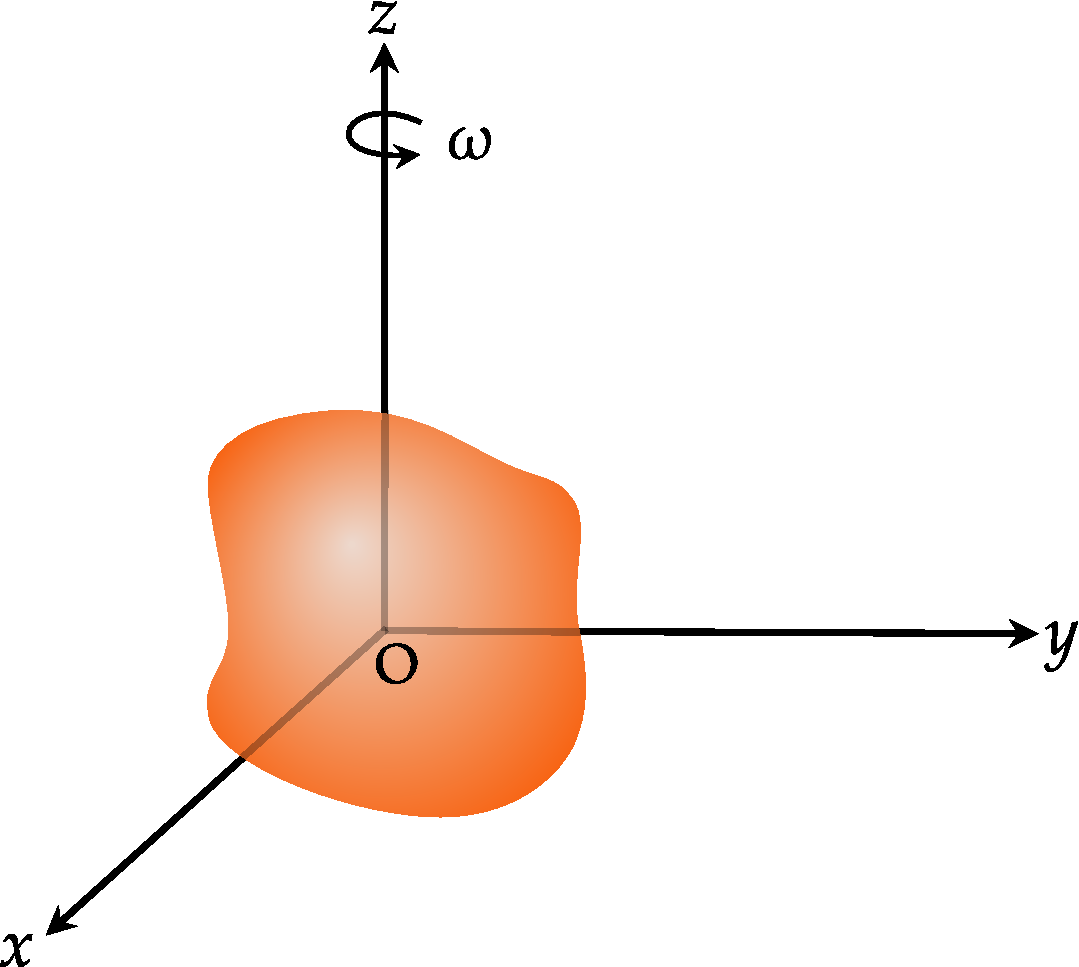
\includegraphics[height=6cm,width=6cm]{rigidbody angularmomentum}
	\end{minipage}
\begin{minipage}{0.45\textwidth}
\centering
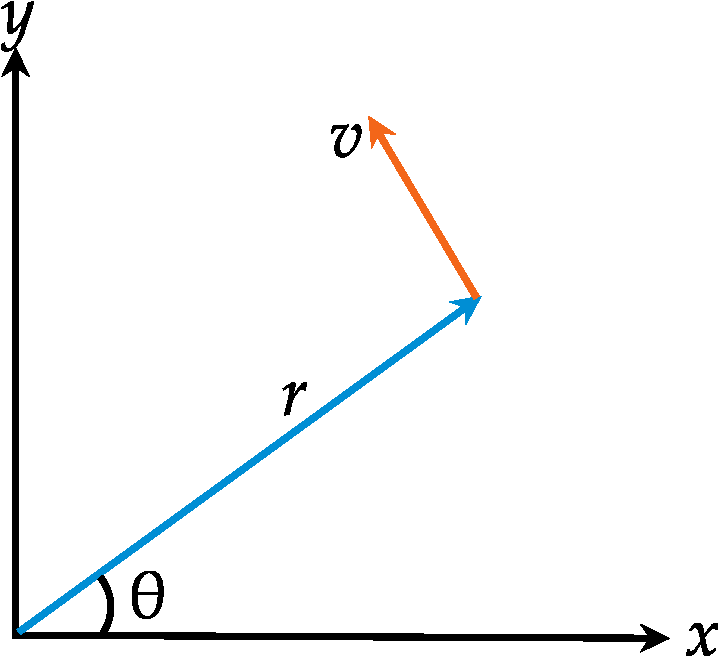
\includegraphics[height=4cm,width=4cm]{rigidbody angularmomentum 1}
\end{minipage}
\caption{Fixed axis rotation of rigid body}
\label{Fixed axis rotation}
\end{figure}
The rigid body pivoted at the origin and rotates with angular speed $\omega$ around the $z$ axis, in the counterclockwise direction (as viewed from above). Consider a little piece of the body, with mass $d m$ and position $(x, y)$. This little piece travels in a circle around the origin with speed
\begin{align*}
v&=\omega r\\
\text{Where,}\ r&=\sqrt{x^{2}+y^{2}} \qquad \because x=r\cos\theta \ ;\  y=r\sin\theta
\intertext{Then, the angular momentum of this piece (relative to the origin) equals}
\mathrm{J}&=\mathrm{r} \times \mathrm{p}\\&=r(v d m) \hat{\mathrm{z}}\\&=d m r^{2} \omega \hat{\mathrm{z}}
\intertext{Then the angular momentum of the entire body is therefore}
\mathrm{J}&=\int r^{2} \omega \hat{\mathrm{z}} d m\\&=\int\left(x^{2}+y^{2}\right) \omega \hat{\mathrm{z}} d m
\intertext{Where the integration runs over the area of the body. If the density of the object is constant, as is usually the case, then we have,}
d m&=\rho d x d y
\intertext{If we define the moment of inertia around the $z$ axis to be}
I_{z} &= \int r^{2} d m\\&=\int\left(x^{2}+y^{2}\right) d m
\intertext{Then the $z$ component of the angular momentum}
J_{z}&=I_{z} \omega\\
\text{And in general, the moment of inertia,}\quad I_{z}&= \sum_{i} m_{i} r_{i}^{2}
\end{align*}
\begin{center}
	\framebox{
		\parbox[t][2.5cm]{4cm}{
			
			\addvspace{0.2cm} \centering 
			
	
	\begin{align*}
	I&= \sum_{i} m_{i} r_{i}^{2}\\
	J&= I\omega
	\end{align*}} }
\end{center}
\subsection{Torque}
Torque about a point is defined as the rate of change of angular momentum about the same point.
\begin{align*}
\tau&=\frac{dJ}{dt}
\intertext{For a rigid body rotating about it's axis of symmetry}
\tau&=\frac{d (I\omega)}{dt}\\&=I \frac{d \omega}{dt}
\intertext{$\frac{d \omega}{dt}$\ is the angular acceleration.}
\intertext{\textbf{Case-1: } If the axis of rotation and axis of symmetry of the bbody are not one. $J$ and $\omega $ may not along the same direction. Then,}
\tau_{0}&=\frac{d (I\omega)}{dt}
\intertext{\textbf{Case-2: } If the axis of rotation fixed relative to the body . $I$ will be constant. Then,}
\tau_{0}&=I\frac{d \omega}{dt}
\intertext{In the absence of external torque $\tau=0$. Then the angular momentum about the axis of rotation is conserved. }
I\omega&= \text{Constant.}
\end{align*}
\section{Moment of Inertia tensor}
particle $P$ of the body, having the position vector $r_{i}$ with respect to $O$, has an instantaneous velocity $v_{i}$ relative to $O$, given by
\begin{align}
\mathbf{v}_{i}&=\omega \times \mathbf{r}_{i}
\intertext{The angular velocity $\omega$ has components $\omega_{x}, \omega_{y}, \omega_{z}$ along $x$, $y$ and  $z$ axes . }
\omega&=\omega_{x} \hat{\mathrm{i}}+\omega_{y} \hat{\mathrm{j}}+\omega_{z} \hat{\mathrm{k}}
\intertext{Then the angular momentum is given by,}
\mathrm{J}_{p}&=\mathrm{r}_{i} \times m_{i} \mathrm{v}_{i} \quad \text{$\mathrm{m}_{i}$ is the  mass of the particle.}
\intertext{Then the angular momentum ,}
\mathrm{J}&=\sum_{i=1}^{N} \mathrm{r}_{i} \times m_{i} \mathrm{v}_{i}\\&=\sum_{i} m_{i} \mathrm{r}_{i} \times\left({\omega} \times \mathrm{r}_{i}\right)\\
&=\sum_{i} m_{i}\left[\left(\mathrm{r}_{i} \cdot \mathrm{r}_{i}\right) \omega-\left(\mathrm{r}_{i} \cdot \omega\right) \mathrm{r}_{i}\right] \\
&=\sum_{i} m_{i}\left[\mathrm{r}_{i}^{2} \omega-\left(\mathrm{r}_{i} \cdot \omega\right) \mathrm{r}_{i}\right]
\intertext{Whose direction is not along that of angular velocity If $J_{x}, J_{y}, J_{z}$ are the components of angular momentum along $X, Y, Z$ axes respectively, then}
J_{x}&=\sum_{i} m_{i}\left[r_{i}^{2} \omega_{x}-\left(x_{i} \omega_{x}+y_{i} \omega_{y}+z_{i} \omega_{z}\right) x_{i}\right]
\intertext{It can be written as,}
\begin{split}
J_{x}&=\omega_{x} \sum_{i} m_{i}\left(r_{i}^{2}-x_{i}^{2}\right)-\omega_{y} \sum_{i} m_{i} x_{i} y_{i}-\omega_{z} \sum_{i} m_{i} x_{i} z_{i} \\
J_{y}&=-\omega_{x} \sum_{i} m_{i} x_{i} y_{i}+\omega_{y} \sum_{i} m_{i}\left(r_{i}^{2}-y_{i}^{2}\right)-\omega_{z} \sum m_{i} y_{i} z_{i} \\
J_{z}&=-\omega_{x} \sum_{i} m_{i} x_{i} z_{i}-\omega_{y} \sum_{i} m_{i} y_{i} z_{i}+\omega_{z} \sum_{i} m_{i}\left(r_{i}^{2}-z_{i}^{2}\right)
\end{split}\\\\
\begin{split}
J_{x}&=I_{x x} \omega_{x}+I_{x y} \omega_{y}+I_{x z} \omega_{z} \\
J_{y}&=I_{y x} \omega_{x}+I_{y y} \omega_{y}+I_{y z} \omega_{z} \\
J_{z}&=I_{z x} \omega_{x}+I_{z y} \omega_{y}+I_{z z} \omega_{z}
\end{split}
\intertext{Where,}
\begin{split}
I_{x x}&=\sum_{i} m_{i}\left(r_{i}^{2}-x_{i}^{2}\right)=\sum_{i} m_{i}\left(y_{i}^{2}+z_{i}^{2}\right) \\
I_{y y}&=\sum_{i} m_{i}\left(r_{i}^{2}-y_{i}^{2}\right)=\sum_{i} m_{i}\left(\dot{x}_{i}^{2}+z_{i}^{2}\right)\\
I_{z z}&=\sum_{i} m_{i}\left(r_{i}^{2}-z_{i}^{2}\right)=\sum_{i} m_{i}\left(x_{i}^{2}+y_{i}^{2}\right)
\end{split}
\intertext{And,}\
\begin{split}
I_{x y}&=-\sum_{i} m_{i} x_{i} y_{i}=I_{y x} \\
I_{x z}&=-\sum_{i} m_{i} x_{i} z_{i}=I_{z x} \\
I_{y z}&=-\sum_{i} m_{i} y_{i} z_{i}=I_{z y}
\end{split}
\intertext{Then any component of the angular momentum vector can be written as,}
J_{\alpha}&=\sum_{\beta} I_{\alpha \beta} \omega_{\beta} \quad \text { Where } \alpha, \beta=x, y, z\\
\text{Or }\ J&= I\omega
\intertext{In matrix notation,}
\left[\begin{array}{c}
J_{x} \\
J_{y} \\
J_{z}
\end{array}\right]&=\left[\begin{array}{lll}
I_{x x} & I_{x y} & I_{x z} \\
I_{y x} & I_{y y} & I_{y z} \\
I_{z x} & I_{z y} & I_{x z}
\end{array}\right] \left[\begin{array}{l}
\omega_{x} \\
\omega_{y} \\
\omega_{z}
\end{array}\right]
\intertext{The nine elements $I_{x x}, I_{x y}, \ldots, I_{x z}$ of the $(3 \times 3)$ matrix may be regarded as components of a single entity $I$. This entity $I$ is called inertia tensor. Since $I_{x y}=I_{y x}$ etc., $I$ is a symmetric tensor.}
I&= \left[\begin{array}{lll}
I_{x x} & I_{x y} & I_{x z} \\
I_{y x} & I_{y y} & I_{y z} \\
I_{z x} & I_{z y} & I_{x z}
\end{array}\right] 
\end{align}
\section{Principle axes and Principle moment of inertia}
If  a body  has  symmetries  with  respect  to  some  of  the  axis,  then  some  of  the  products  of  inertia  become  zero  and  we  can  identify  the  principal  axes.   If  a  body  is  symmetric  with  respect  to  the plane $x^{\prime}=0$ then, we will have $I_{x^{\prime} y^{\prime}}=I_{y^{\prime} x^{\prime}}=I_{x^{\prime} z^{\prime}}=I_{z^{\prime} x^{\prime}}=0$ and $x^{\prime}$ will be a principal axis. 
\\If we choose the axes of the coordinate system fixed in the body with respect to which \textbf{off-diagonal elements disappear and only the diagonal elements remain in the inertia tensor, then such axes are called the principal axes} of the body and the corresponding moments of inertia as the principal moments of inertia. In general the directions of the principal axes are different to those of arbitrary axes fixed in the body. If $x^{\prime}$ , $y^{\prime}$ and $z^{\prime}$ are the principle axes then the principle moment of inertia can be written as, 
\begin{equation}
{I}=\left[ \begin{array}{ccc}
I_{1} & 0 & 0 \\
0 & I_{2} & 0 \\
0 & 0 & I_{3}
\end{array}\right]
\end{equation}
Where, $I_{x^{\prime} x^{\prime}}=I_{1}, I_{y^{\prime} y^{\prime}}=I_{2} \text { and } I_{z z^{\prime}}=I_{3}$
\\If $\omega_{1}, \omega_{2}, \omega_{3}$ be the components of angular velocity and $J_{1}, J_{2}, J_{3}$ those of angular momentum about the principal axes, then  for the principal axes  we obtain the angular momenta as,
\begin{align}
\left(\begin{array}{l}
J_{1} \\
J_{2} \\
J_{3}
\end{array}\right)&=\left(\begin{array}{lll}
I_{1} & 0 & 0 \\
0 & I_{2} & 0 \\
0 & 0 & I_{3}
\end{array}\right)\left(\begin{array}{l}
\omega_{1} \\
\omega_{2} \\
\omega_{3}
\end{array}\right)
\end{align}

\section{Parallel and perpendicular axes theorem}
\subsection{ Theorem of Parallel Axis }
Consider a rigid body of mass $M$ undergoing fixed-axis rotation. 
\begin{theorem}
According to the theorem of parallel axis, the moment of inertia of a body about any axis is equal to the sum of moment of inertia about a parallel axis through it's center of mass and the product of the mass of the body and the square of the distance between two axes.
\begin{equation}
I= I_{cm}+M d^{2}
\end{equation}
\begin{align*}
\text{Where,}\qquad I&= \text{Moment of inertia about any axis.}\\
I_{cm}&= \text{Moment of inertia of the body about a parallel axis passing through it's center of mass.}\\
m&= \text{Mass of the body.}\\
d&= \text{Distance between the two axes.}\\
\end{align*}
\end{theorem}
\subsection{Theorem of Perpendicular Axis}
\begin{theorem}
According to the theorem of perpendicular axis, the moment of inertia of a plane lamina about an axis perpendicular to it's plane is equal to the sum of moments of inertia of the lamina about two axes  at right angles to each other, in it's own plane, and intersecting each other at the point where the perpendicular axis passes through it.\\
If  $I_{\mathrm{x}}$  and $I_{\mathrm{y}}$ be the moment of inertia of a plane lamina about $x$ and $y$ axes . Which lie in the palne of the lamina  and mutually peroendicular to each other intersecting at the origin. The n the moment of inertia  $I$ about an axis which is passing through the origin and perpendicular to the oplane of the lamina is ,
\begin{equation}
I=I_{\mathrm{x}}+I_{\mathrm{y}}
\end{equation}
\end{theorem}

\section{Moment of Inertia of some simple objects}

\subsection{Moment of Inertia of a thin uniform rod }
\subsubsection{1. About an axis passing through the center of mass and perpendicular to it's length.}
Consider a thin uniform rod of length $L$ and mass $m$ and uniform mass density $\lambda$.  Choose Cartesian coordinates, with the origin at the center of mass of the rod, which is midway between the endpoints since the rod is uniform. Choose the $x$-axis to lie along the length of the rod, with the positive $x$-direction to the right, as in the figure.\ref{Uniform rod}
\begin{figure}[H]
	\centering
	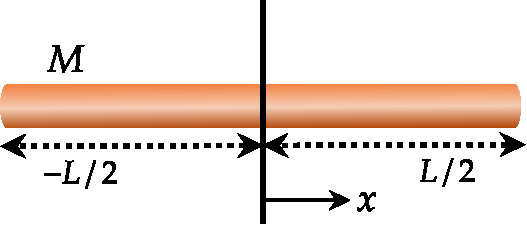
\includegraphics[height=1.8cm,width=4cm]{MI rod 1}
	\caption{Uniform rod with an axis passing through the center.}
	\label{Uniform rod}
\end{figure}
\begin{align*}
\intertext{Consider an infinitesimal mass element  $dm$ ,located at a displacement  $x$  from the 
	center  of  the  rod,, } \ dm&= \lambda dx \qquad \text{Where,}\ \lambda=\frac{m}{L}
\intertext{The moment of inertia of a continuos mass distribution is given by,}\ I&= \int r^{2} d m\\
\text{Then,}\ I&=\int_{-L/2}^{L/2} x^{2} \frac{m}{L}dx\\&= \frac{m}{L} \int_{-L/2}^{L/2} x^{2} dx\\&=
\frac{m}{L} \left[\frac{x^{3}}{3} \right]_{-L/2}^{L/2} =\frac{m}{3L} \frac{2L^{3}}{8} \\&=\frac{1}{12}mL^{2}
\end{align*}
\subsubsection{2.  About an axis passing  through  the  endpoint. }
\begin{figure}[H]
	\centering
	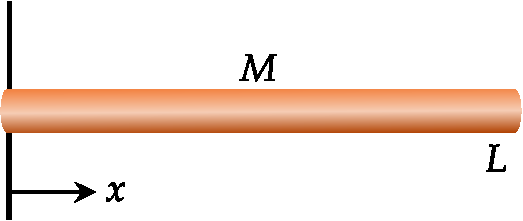
\includegraphics[height=1.8cm,width=4cm]{MI rod 2}
	\caption{Uniform rod with an axis passing through the end point.}
	\label{Uniform rod}
\end{figure}
According to the theorem of parallel axis, the moment of inertia about any axis is given by,
\begin{align*}
I&= I_{cm}+M d^{2}\quad  \text{Where $d$ is the distance from the axis to center of mass .}\\
\text{Here,}\quad d&=\frac{L}{2}\\
I&=\frac{1}{12} m L^{2}+\frac{1}{4} m L^{2}\\&=\frac{1}{3} m L^{2} 
\end{align*}
\subsection{Moment of Inertia of a Uniform Disc}
\subsubsection{1. About an axis passing through the center of mass and perpendicular to the plane of the disc.}

\begin{figure}[H]
\begin{minipage}{0.45\textwidth}
   \centering
	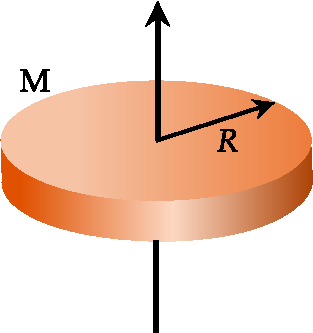
\includegraphics[height=4cm,width=4cm]{MI disc 1}
\end{minipage}
\begin{minipage}{0.45\textwidth}
 \centering
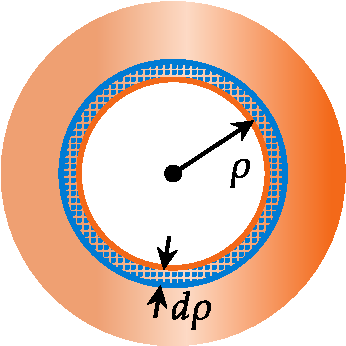
\includegraphics[height=3cm,width=3cm]{MI disc 2}
\end{minipage}
\caption{Uniform Disc with an axis passing through the center of mass}
\label{}
\end{figure}
Choose cylindrical coordinates with the coordinates $(r, \theta)$ in the plane and the $z$-axis perpendicular to the plane. The area element,
\begin{align*}
d a&=\rho d \rho d \theta\\
\sigma &= \frac{M}{A}=\frac{M}{\pi R^{2}}
\intertext{ The infinitesimal mass }\ 
d m &= \frac{M}{A} d a\\&=\frac{M}{\pi R^{2}} \rho d \rho d \theta 
\intertext{Then the moment of inertia ,} \ I &=\int \rho^{2} \sigma d a \\
&=\left(\frac{M}{\pi R^{2}}\right) \int \rho^{2} d a \\
&=\left(\frac{M}{\pi R^{2}}\right) \int_{0}^{R} \int_{0}^{2 \pi} \rho^{2} \rho d \rho d \theta \\
&=\left(\frac{2 M}{R^{2}}\right) \int_{0}^{R} \rho^{3} d \rho \\
&=\frac{1}{2} M R^{2}
\end{align*}
\subsubsection{2. About an axis passing through the diameter.}
\begin{figure}[H]
	\centering
	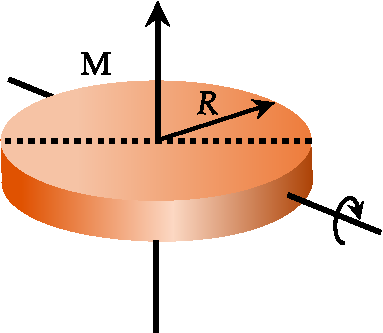
\includegraphics[height=3cm,width=4cm]{MI disc 4}
	\caption{Uniform disc with an axis passing through the diameter.}
	\label{}
\end{figure}
By the theorem of perpendicular axis,
\begin{align*}
I_{z}&=I_{x}+I_{y}
\intertext{The moment of inertia of the disc is the same about any diameter. Let I be the moment of inertia about any diameter $xx^{\prime}$. Then it will be the moment of inertia  about a perpendicular diameter  $yy^{\prime}$}
\text{Here,}\ I_{z}&=\frac{M R^{2}}{2}\\
\text{And ,}\ I_{x}&=I_{y}=I\\
\frac{M R^{2}}{2}&= 2I\\
 I&= \frac{M R^{2}}{4}
\end{align*}
\subsection{Moment of inertia of a solid sphere .}
\subsubsection{1. About an axis passing through the diameter.}
\begin{align*}
\text{The volume element,}\ dv&= r^{2}dr \sin \theta  d\theta d\phi \\\text{The infinitesimal mass element,} \ dm &=\frac{M}{V} dv\\
&=\frac{M}{\frac{4}{3} \pi R^{3}} r^{2}dr \sin \theta  d\theta d\phi\\
\text{Here, }\ r_{\perp}&=r\sin\theta\\
I&=\int r_{\perp}^{2}+d m\\&=\iiint r^{2} \sin ^{2} \theta \cdot \frac{M}{\frac{4}{3} \pi R^{3}} r^{2} d r \sin \theta d \theta d \phi\\&=\frac{3 M}{4 \pi R^{3}} \int_{0}^{R} r^{4} d r \int_{0}^{\pi} \sin ^{3} \theta d \theta \int_{0}^{2 \pi} d \phi\\
&=\frac{3 M}{4 \pi R^{3}} \cdot \frac{R^{5}}{5} \cdot \frac{4}{3} \cdot 2 \pi\\&=\frac{2}{5} M R^{2}
\end{align*}
\subsubsection{2. About an axis passing through it's tangent.}
\begin{minipage}{0.45\textwidth}
\begin{figure}[H]
	\centering
	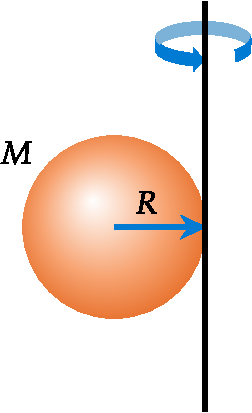
\includegraphics[height=5cm,width=3cm]{mi solid 1}
	\caption{About an axis passing through it's tangent.}
	\label{About an axis passing through it's tangent.}
\end{figure}
\end{minipage}\hfill
\begin{minipage}{0.45\textwidth}
	\begin{figure}[H]
		\centering
		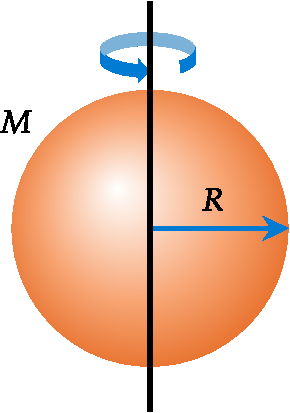
\includegraphics[height=4cm,width=3cm]{mi solid 2}
		\caption{About an axis passing through it's diameter.}
		\label{About an axis passing through it's diameter.}
	\end{figure}
\end{minipage}\\\\
Any tangent to the sphere at any point is parallel to one of it's diameter and is at  a distance equal to $R$ from the centre.  Now by the application of the theorem of parallel axis  the moment of inertia becomes,
\begin{align*}
\intertext{According to the theorem of parallel axis, the moment of inertia about any axis is given by,}
I&= I_{cm}+M d^{2}\quad  \text{Where $d$ is the distance from the axis to center of mass .}\\
\text{Here,}\quad d&=R\\
I&=\frac{2}{5} m R^{2}+m R^{2}\\&=\frac{7}{5} m R^{2} 
\end{align*}
\subsection{Moment of inertia of a spherical shell.}
\subsubsection{1. About an axis passing through it's diameter.}
On the spherical shell the mass element is ,
\begin{align*}
da&= R^{2} \sin \theta d\theta d \phi\\
\sigma&= \frac{M}{a}\\
d m&=\sigma R \sin \theta d \theta R d \phi
\intertext{where $\sigma=M / 4 \pi R^{2}$ is the surface mass density, and the distance from the rotational axis is $r=R \sin \theta$. Hence the moment of inertia to be calculated is}
I&=\int r_{\perp}^{2}+d m\\&=\iint R^{2} \sin ^{2} \theta \cdot \frac{M}{{4}\pi R^{2}} R^{2}  \sin \theta d \theta d \phi\\&=\frac{M R^{2}}{4 \pi }  \int_{0}^{\pi} \sin ^{3} \theta d \theta \int_{0}^{2 \pi} d \phi\\
&=\frac{ M R^{2}}{4 \pi} \cdot  \frac{4}{3} \cdot 2 \pi\\&=\frac{2}{3} M R^{2}
\end{align*}
\begin{minipage}{0.45\textwidth}
\begin{figure}[H]
	\centering
	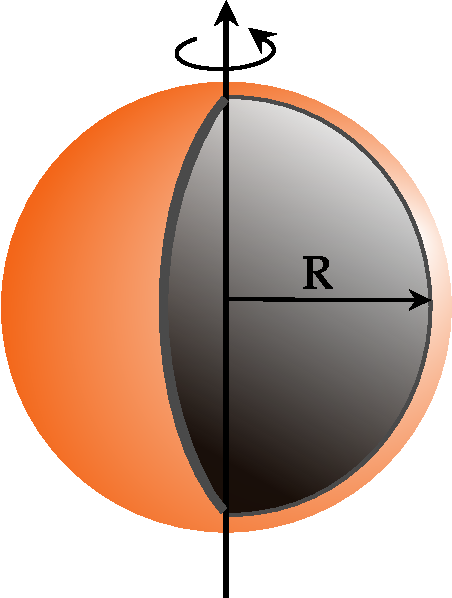
\includegraphics[height=4cm,width=3cm]{mi spherical shell}
	\caption{About an axis passing through it's diameter.}
	\label{About an axis passing through it's diameter.}
\end{figure}
\end{minipage}\hfill
\begin{minipage}{0.45\textwidth}
\begin{figure}[H]
	\centering
	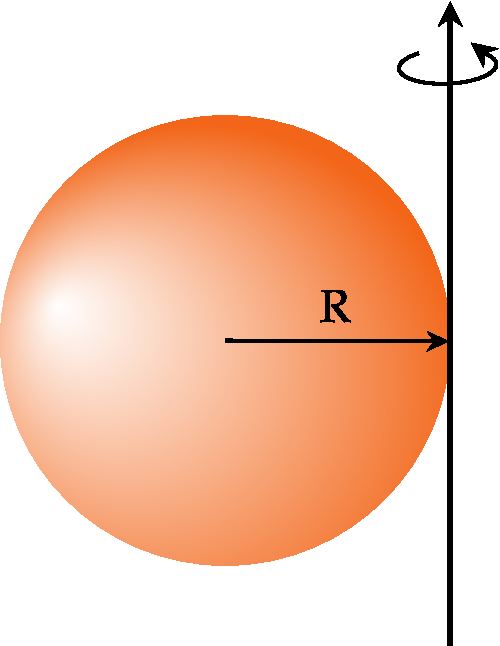
\includegraphics[height=4cm,width=3cm]{mi hollow spherical 2}
	\caption{About an axis passing through it's tangent.}
	\label{About an axis passing through it's tangent.}
\end{figure}
\end{minipage}
\subsubsection{2. About an axis passing through it's tangent.}
Any tangent to the sphere at any point is parallel to one of it's diameter and is at  a distance equal to $R$ from the centre.  Now by the application of the theorem of parallel axis  the moment of inertia becomes,
\begin{align*}
\intertext{According to the theorem of parallel axis, the moment of inertia about any axis is given by,}
I&= I_{cm}+M d^{2}\quad  \text{Where $d$ is the distance from the axis to center of mass .}\\
\text{Here,}\quad d&=R\\
I&=\frac{2}{3} m R^{2}+m R^{2}\\&=\frac{5}{3} m R^{2} 
\end{align*}
\section{Kinetic energy of a rotating body}
The kinetic energy of a rotating body about an axis depends not only upon it's mass and angular velocity but also depends upon the position of the axis and the distribution of mass about that axis.
Suppose a body of mass $M$ is rotating about an axis . Assume that the body is a system of small particles . 
\begin{align*}
\intertext{Let us consider a particle $P$ of elementary mass $m$ at a distance $r$ from the axis.}
\text{The angular velocity}&=\omega\\
\text{The linear velocity }&=r \omega
\intertext{Then the kinetic energy of rotation,}
\text{K.E}&=\frac{1}{2} m r^{2} \omega^{2} 
\intertext{Hence the kinetic energy (K.E.) of rotation of the whole body is given by,}
E&=\Sigma \frac{1}{2} m r^{2} \omega^{2}\\&=\frac{1}{2} \omega^{2} \Sigma m r^{2}\\
\text{Now,} \  \Sigma m r^{2}&=I \quad \text{ The moment of inertia about the  given axis}
\intertext{Then the kinetic energy of rotation,} E&=\frac{1}{2} I \omega^{2}\\
\text{If} \ \omega&=1, \text{Obviously}\ I=2  E
\intertext{Hence the moment of inertia of a body may also be defined as twice its kinetic energy of rotation,}
\text{But angular momentum} J&=I \omega \quad \text{where $J$ is along the axis of rotation}\\
\therefore \quad J&=I\sqrt{2 E / I}=\sqrt{2 E I} \\
\text { or } E&=J^{2} / 2 I
\intertext{This is the relation between rotational kinetic energy and angular momentum on the same aaxis}
\end{align*} 
\newpage
\colorlet{ocre1}{ocre!70!}
\colorlet{ocrel}{ocre!30!}
\setlength\arrayrulewidth{1pt}
\begin{table}[H]
	\centering
	\arrayrulecolor{ocre}
	\renewcommand*{\arraystretch}{1.5}
	\begin{tabular}{|p{4cm}|p{6cm}|p{3cm}|}
		\hline
		\multicolumn{3}{|c|}{\textbf{Center of mass of uniform systems}}\\\hline\hline
		\rowcolor{ocrel}Uniform body& & Moment of Inertia\\\hline
		Thin Rod (About center)&
		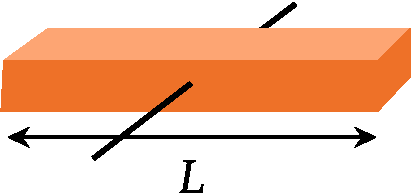
\includegraphics[height=1.5cm,width=3.5cm]{moment i 1}
		&\textbf{$\frac{1}{12}ML^{2}$}   \\\hline 
		Thin Rod (About End)& 			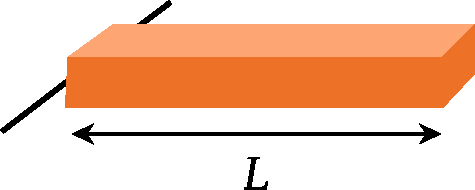
\includegraphics[height=1.5cm,width=3.5cm]{moment i 2} & \textbf{$\frac{1}{2}ML^{3}$}   \\\hline 
		Rectangular plane (About center)& 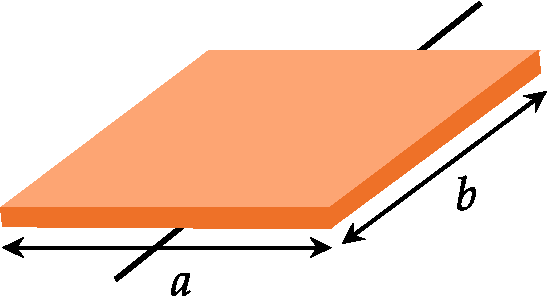
\includegraphics[height=2.5cm,width=4cm]{ moment i 3} &\textbf{$\frac{1}{12}Ma^{2}$}   \\\hline 
		Rectangular plane (About Edge)&	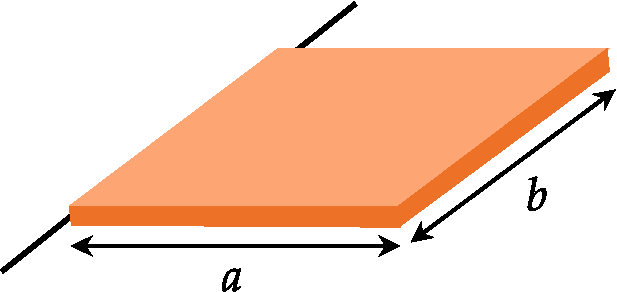
\includegraphics[height=2.5cm,width=4cm]{ moment i 4} & \textbf{$\frac{1Ma^{2}}{2}$}   \\\hline 
		Cylinder& 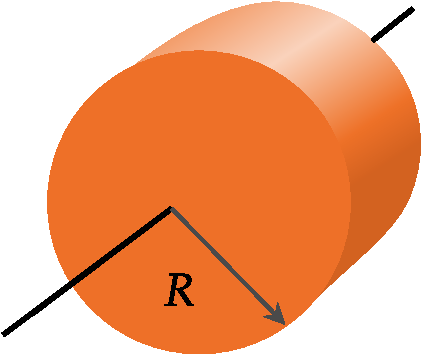
\includegraphics[height=2.5cm,width=3cm]{moment i 5} &\textbf{$\frac{1}{2}MR^{2}$}   \\\hline
		Cylindrical hoop& 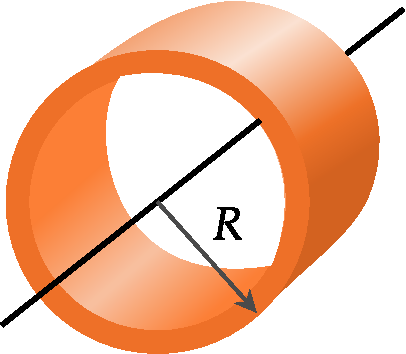
\includegraphics[height=2.5cm,width=3cm]{moment i 6} &\textbf{$MR^{2}$}   \\\hline
		Solid sphere(About diameter)& 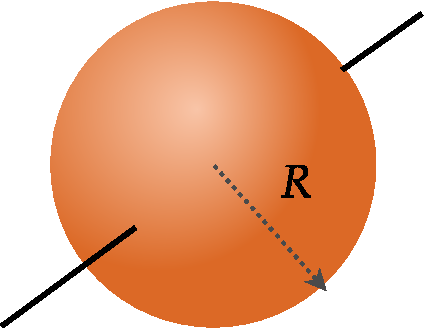
\includegraphics[height=2.5cm,width=3.2cm]{moment i 7} &\textbf{$\frac{2}{3}MR^{2}$}   \\\hline
		Spherical shell (About diameter)& 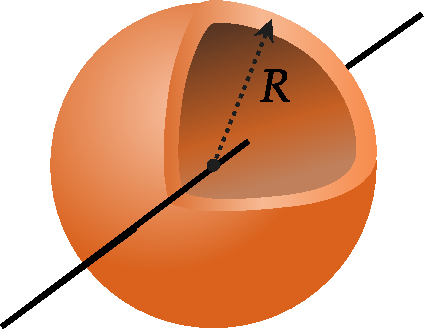
\includegraphics[height=2.5cm,width=3.2cm]{moment i 8} &\textbf{$\frac{2}{5} MR^{2}$}   \\\hline
	\end{tabular}
\end{table}
\newpage
\begin{abox}
Practice set 1
\end{abox}
\begin{enumerate}
\begin{minipage}{\textwidth}
	\item An annulus of mass $M$ made of a material of uniform density has inner and outer radii $a$ and $b$ respectively. Its principle moment of inertia along the axis of symmetry perpendicular to the plane of the annulus is:
	\exyear{NET DEC 2011}
\end{minipage}
\begin{tasks}(2)
	\task[\textbf{A.}] $\frac{1}{2} M \frac{\left(b^{4}+a^{4}\right)}{\left(b^{2}-a^{2}\right)}$
	\task[\textbf{B.}]$\frac{1}{2} M \pi\left(b^{2}-a^{2}\right)$
	\task[\textbf{C.}]$\frac{1}{2} M\left(b^{2}-a^{2}\right)$
	\task[\textbf{D.}]$\frac{1}{2} M\left(b^{2}+a^{2}\right)$
\end{tasks}
\begin{minipage}{\textwidth}
	\item Two bodies of equal mass $m$ are connected by a massless rigid rod of length $l$ lying in the $x y$-plane with the centre of the rod at the origin. If this system is rotating about the $z$-axis with a frequency $\omega$, its angular momentum is
	\exyear{NET DEC 2012}
\end{minipage}
\begin{tasks}(2)
	\task[\textbf{A.}] $m l^{2} \omega / 4$
	\task[\textbf{B.}]$m l^{2} \omega / 2$
	\task[\textbf{C.}]$m l^{2} \omega$
	\task[\textbf{D.}]$2 m l^{2} \omega$
\end{tasks}
\begin{minipage}{\textwidth}
	\item Two masses $m$ each, are placed at the points $(x, y)=(a, a)$ and $(-a,-a)$ and two masses, $2 m$ each, are placed at the points $(a,-a)$ and $(-a, a)$. The principal moments of inertia of the system are
	\exyear{NET DEC 2015}
\end{minipage}
\begin{tasks}(2)
	\task[\textbf{A.}] $2 m^{2}, 4 m a^{2}$
	\task[\textbf{B.}]$4 m a^{2}, 8 m a^{2}$
	\task[\textbf{C.}] $4 m a^{2}, 4 m a^{2}$
	\task[\textbf{D.}] $8 m a^{2}, 8 m a^{2}$
\end{tasks}
\begin{minipage}{\textwidth}
	\item A disc of mass $m$ is free to rotate in a plane parallel to the $x y$ plane with an angular velocity $-\omega \hat{z}$ about a massless rigid rod suspended from the roof of a stationary car (as shown in the figure below). The rod is free to orient itself along any direction.
	\begin{figure}[H]
		\centering
		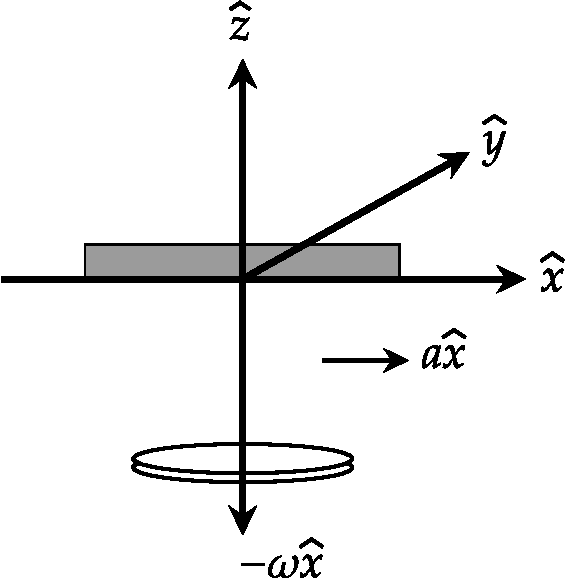
\includegraphics[height=4cm,width=5cm]{diagram-20210926(37)-crop}
	\end{figure}
	The car accelerates in the positive $x$-direction with an acceleration $a>0 .$ Which of the following statements is true for the coordinates of the centre of mass of the disc in the reference frame of the car?
	\exyear{NET DEC 2017}
\end{minipage}
\begin{tasks}(2)
	\task[\textbf{A.}] only the $x$ and the $z$ coordinates change
	\task[\textbf{B.}]only the $y$ and the $z$ coordinates change
	\task[\textbf{C.}]only the $x$ and the $y$ coordinates change
	\task[\textbf{D.}]all the three coordinates change
\end{tasks}
\end{enumerate}


\newpage
\begin{abox}
	Practice set 2
	\end{abox}
\begin{enumerate}
\begin{minipage}{\textwidth}
	\item A uniform solid cylinder is released on a horizontal surface with speed $5 \mathrm{~m} / \mathrm{s}$ without any rotation (slipping without rolling). The cylinder eventually starts rolling without slipping. If the mass and radius of the cylinder are $10 \mathrm{gm}$ and $1 \mathrm{~cm}$ respectively, the final linear velocity of the cylinder is.............. $\mathrm{m} / \mathrm{s}$. (up to two decimal places).
	\exyear{GATE 2017}
\end{minipage}
\begin{minipage}{\textwidth}
	\item A uniform circular disc of mass $m$ and radius $R$ is rotating with angular speed $\omega$ about an axis passing through its centre and making an angle $\theta=30^{\circ}$ with the axis of the disc. If the kinetic energy of the disc is $\alpha m \omega^{2} R^{2}$, the value of $\alpha$ is (up to two decimal places).
	\exyear{GATE 2018}
	\begin{figure}[H]
		\centering
		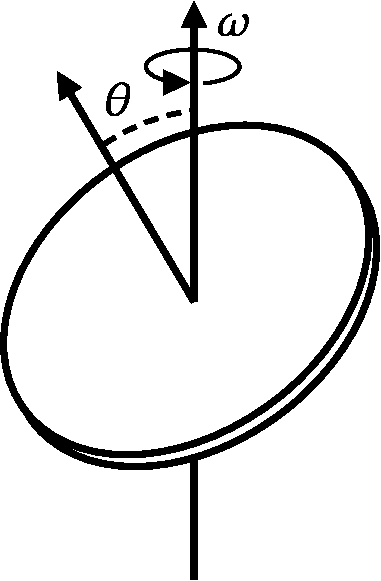
\includegraphics[height=3cm,width=3cm]{diagram-20210915(17)-crop}
	\end{figure}
\end{minipage}
\end{enumerate}


\newpage
\begin{abox}
	Practice set-3
\end{abox}
\begin{enumerate}[label=\color{ocre}\textbf{\arabic*.}]
	\item Show that the centre of mass of a rod of mass $M$ and length L lies midway between its ends, assuming the rod has a uniform mass per unit length.\\
	\begin{figure}[H]
		\centering
		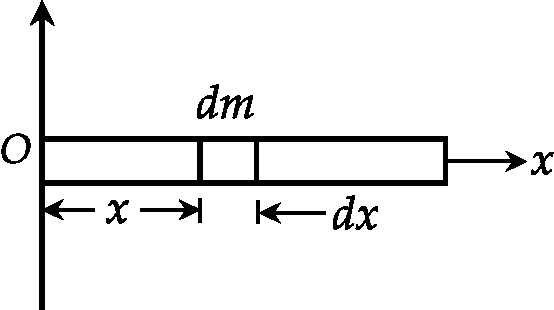
\includegraphics[height=3cm,width=5cm]{fm14}
	\end{figure}
	\begin{answer}
		By symmetry, we see that $y_{C M}=z_{C M}=0$ if the rod is placed along the $x$ axis. Furthermore, if we call the mass per unit length $\lambda$ (the linear mass density), then $\lambda=\mathrm{M} / \mathrm{L}$ for a uniforr rod.
		If we divide the rod into elements of length $d x$, then the mass of each element is $\mathrm{dm}=? \mathrm{dx}$. Since an arbitrary element of each element is at a distance $x$ from the origin, equation gives,
		\begin{align*}
		x_{C M}&=\frac{1}{M} \int_{0}^{L} x d m\\&=\frac{1}{M} \int_{0}^{L} x \lambda d x\\&=\frac{\lambda L^{2}}{2 M}\\
		\text{Because }\lambda&=M / L \ \text{ this reduces to,}\ x_{C M}=\frac{L^{2}}{2 M}\left(\frac{M}{L}\right)=\frac{L}{2}
		\intertext{One can also argue that by symmetry,} \ x_{C M}&=\frac{L }{2}
		\end{align*}
	\end{answer}
	\item $A$ body of radius $R$ and mass $M$ is rolling horizontally without slipping with speed $v$, it then rolls $u p$ a hill to a maximum height $h .$ If $h=3 v^{2} / 4 \mathrm{~g}$, \\(a) what is the moment of inertia of the body? \\(b) what might be the shape of the body?
\begin{answer}
	\begin{align*}
	\text{(a)}\quad \mathrm{K}_{\text {total }}&=\mathrm{K}_{\text {trans. }}+\mathrm{K}_{\text {rot. }}=\frac{1}{2} \mathrm{M} \mathrm{v}^{2}+\frac{1}{2} \mathrm{I} \omega^{2}\\
	&=\frac{1}{2} M v^{2}+\frac{1}{2} I\left(\frac{v^{2}}{R^{2}}\right)=\frac{v^{2}}{2}\left[M+\frac{I}{R^{2}}\right]
	\intertext{When it rolls up a hill to height $\mathrm{h}$, the entire kinetic energy is converted into potential energy $\mathrm{M} \mathrm{g} \mathrm{h}$}
	\text{Thus} \frac{\mathrm{v}^{2}}{2}\left[\mathrm{M}+\frac{\mathrm{I}}{\mathrm{R}^{2}}\right]&=\mathrm{Mgh}=\mathrm{Mg}\left[3 \frac{\mathrm{v}^{2}}{4 \mathrm{~g}}\right]\\
	\text{or }\left[\mathrm{M}+\frac{\mathrm{I}}{\mathrm{R}^{2}}\right]&=\frac{3}{2} \mathrm{M} \\ \therefore \mathrm{I}&=\frac{\mathrm{MR}^{2}}{2}
	\intertext{\text{(b)}\quad The body may be a circular disc or a solid cylinder.}
	\end{align*}
\end{answer}
	\item Let $g$ be the acceleration due to gravity at earth's surface and $K$ be the rotational kinetic energy of the earth. Suppose the earth's radius decrease by $2 \%$, keeping all other quantities same, then
\begin{tasks}(1)
	\task[\textbf{A.}] g decreases by $2 \%$ and $\mathrm{K}$ decreases by $4 \%$
	\task[\textbf{B.}] g decreases by $4 \%$ and k increases by $2 \%$
	\task[\textbf{C.}] $\mathrm{g}$ increases by $4 \%$ and $\mathrm{K}$ decreases by $4 \%$
	\task[\textbf{D.}] g decreases by $4 \%$ and $\mathrm{K}$ increases by $4 \%$
\end{tasks}
\begin{answer}
	\begin{align*}
	\text{We know that, }g&=\frac{G M}{R^{2}}\\
	\text{Differentiating, }\frac{\mathrm{dg}}{\mathrm{g}}&=-\left(\frac{2 \mathrm{dR}}{\mathrm{R}}\right)\\
	\text{Further, }\mathrm{K}&=\frac{1}{2} \mathrm{I} \omega^{2}=\frac{1}{2}\left[\frac{3}{5} \mathrm{M} \mathrm{R}^{2}\right] \omega^{2}\\
	\text{	or }\frac{\mathrm{dK}}{\mathrm{K}}&=\frac{3}{10} \mathrm{M} \omega^{2} \times\left(\frac{2 \mathrm{dR}}{\mathrm{R}}\right)
	\intertext{When radius decreases by $2 \%$, then $\mathrm{g}$ increases by $4 \%$ and K decreases by $4 \%$.}
	\end{align*}
	So the correct answer is \textbf{Option (C)}
\end{answer}
	\item A cubical block of side $a$ is moving with velocity $v$ on a horizontal smooth plane as shown in fig. It hits a ridge at point $O$. The angular speed of the block after it hits $O$ is\\
\begin{figure}[H]
	\centering
	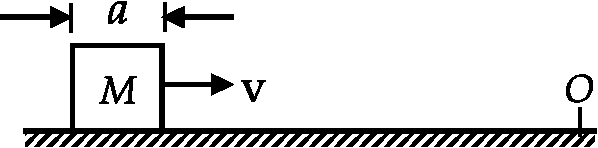
\includegraphics[height=1.5cm,width=5cm]{fm16}
\end{figure}
\begin{tasks}(4)
	\task[\textbf{A.}] $3 \mathrm{v} /(4 \mathrm{a})$
	\task[\textbf{B.}] $3 \mathrm{v} /(2 \mathrm{a})$
	\task[\textbf{C.}] $\sqrt{3} \mathrm{v} /(\sqrt{2} \mathrm{a})$
	\task[\textbf{D.}] Zero
\end{tasks}
\begin{answer}$\left. \right. $\\
	\begin{minipage}{0.65\textwidth}
		\begin{align*}
		\intertext{By conservation of angular momentum, we have}
		I \omega&=M \vee(a / 2)\\
		\text{	Here, }I&=\frac{M a^{2}}{6}+M\left(\frac{a}{\sqrt{2}}\right)^{2}\\&=\frac{2 M a^{2}}{3} \\
		\therefore \frac{2 \mathrm{Ma}^{2}}{3} \omega&=\frac{\mathrm{Mva}}{2} \\ \omega&=\frac{3 \mathrm{v}}{4 \mathrm{a}}
		\end{align*}
	\end{minipage}
	\begin{minipage}{0.35\textwidth}
		\begin{figure}[H]
			\centering
			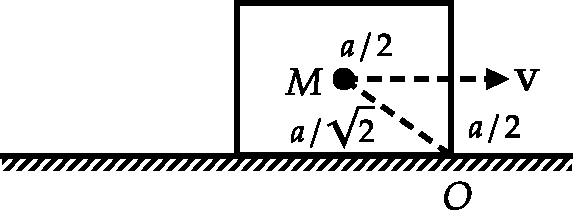
\includegraphics[height=2cm,width=5cm]{fm17}
		\end{figure}
	\end{minipage}
\end{answer}
	\item A sphere is spinned in a clockwise direction by angular velocity $\omega$ and then it is released to a rough surface. Find the time elapsed by the sphere, till it starts pure rolling (coefficient of friction is $\mu$ ) and radius of sphere is $R$.\\
\begin{figure}[H]
	\centering
	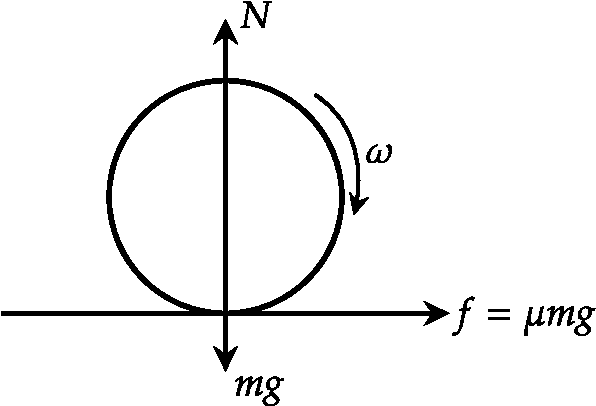
\includegraphics[height=3.3cm,width=5cm]{fm18}
\end{figure}
\begin{answer}
	\begin{align}
	\mathbf{N}&=\mathrm{mg}\notag
	\intertext{$\mathrm{f}=\mu \mathrm{mg}$ (friction opposes relative motion, so it is in forward direction)}\notag\\
	a_{c m}&=\frac{f}{m}=\mu g\label{fm01}\\
	\text{Also }\mathrm{f} \times \mathrm{R}&=\mathrm{I} \alpha\notag\\
	\Rightarrow \mu \mathrm{mgR}&=\mathrm{I} \alpha \Rightarrow \alpha=\frac{\mu \mathrm{mgR}}{\mathrm{I}}=\frac{\mu \mathrm{mgR}}{2 / 5 \mathrm{mR}^{2}}=\frac{5}{2} \frac{\mu \mathrm{g}}{\mathrm{R}}\notag\\
	\omega&=\omega_{\mathrm{o}}-\alpha \mathrm{t}=\omega_{\mathrm{o}}-\frac{5}{2} \frac{\mu \mathrm{gt}}{\mathrm{R}}\label{fm02}
	\intertext{At the instant, $\mathrm{m}$ starts pure rolling}\notag
	\omega R&=v\text{ (lowest point is at rest)}\notag\\
	v_{c m}&=0+\mu g t\label{fm03}
	\intertext{$[$ from eqns. $(\ref{fm02})$ and $(\ref{fm03})$ and $\omega R=v]$}\notag
	\Rightarrow \omega \mathrm{R}&=\frac{7}{2} \mu \mathrm{gt} \Rightarrow \mathrm{t}=\frac{2}{7} \frac{\omega \mathrm{R}}{\mu \mathrm{g}}\notag
	\end{align}
\end{answer}
\item  A uniform solid cube has mass $M$ and side ' $a$ '. Calculate moment of inertia of the cube about an axis which coincides with one of it's sides
\begin{figure}[H]
	\centering
	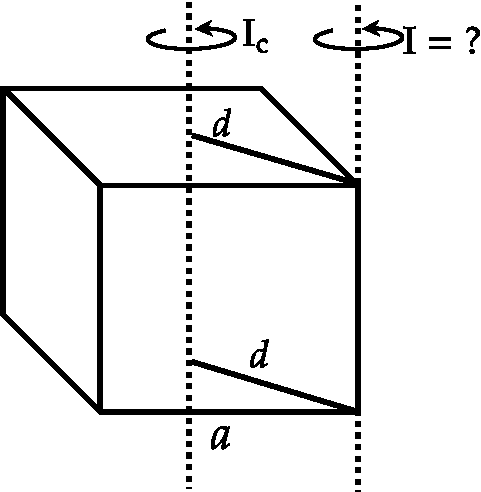
\includegraphics[height=3cm,width=3cm]{Rigid body pset-3}
\end{figure}
\begin{answer}
	\begin{align*}
	\intertext{Moment of inertia of a cube about an axis passing through it's  centre}
	I_{c}&=\frac{Ma^{2}}{6}
	\intertext{Seperation between two axes}
	d&=\frac{a}{\sqrt{2}}
	\intertext{Then according to the parellel axis theorem}
	I&=I_{c}+Md^{2}\\
		&=\frac{Ma^{2}}{6}+M\left( {\frac{a}{\sqrt{2}}}\right) ^{2}\\
		&=\frac{2 Ma^{2}}{3}
	\end{align*}
\end{answer}
 \item A $1 \mathrm{~kg}$ mass of clay, moving with a velocity of 10 $\mathrm{m} / \mathrm{s}$, strikes a stationary wheel and sticks to it. The solid wheel has a mass of $20 \mathrm{~kg}$ and a radius of $1 \mathrm{~m}$.
\begin{figure}[H]
	\centering
	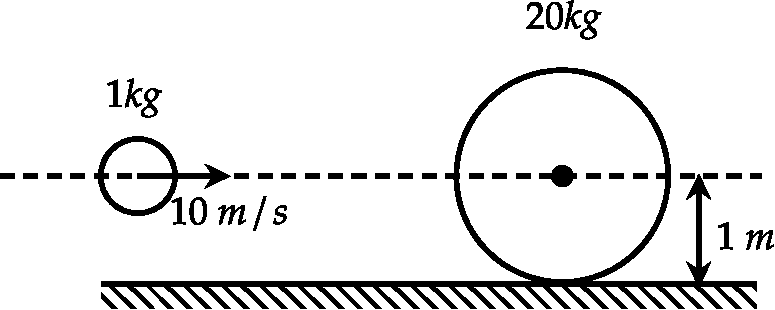
\includegraphics[height=2cm,width=5cm]{mi 1}
	
\end{figure}
 Assuming that the wheel and the ground are both rigid and that the wheel is set into pure rolling motion, the angular velocity of the wheel immediately after the impact is, approximately,
 \begin{tasks}(2)
 	\task[\textbf{a.}]Zero. 
 	\task[\textbf{b.}]$1 / 3 \ \mathrm{rad} / \mathrm{s}$
 	\task[\textbf{c.}]$\sqrt{10 / 3}\  \mathrm{rad} / \mathrm{s}$ 
 	\task[\textbf{d.}]$10 / 3 \ \mathrm{rad} / \mathrm{s}$   
 \end{tasks}
\begin{answer}
	The moment of inertia of wheel of mass $m$ and radius $r$ w.r.t. a normal axis passing through circumference is
	\begin{align*}
	I &=\frac{m r^{2}}{2}+m r^{2} \\
	&=\frac{3}{2} m r^{2}
	\end{align*}
	If $\omega$ is the velocity of pure rolling of wheel after the impact, total kinetic energy of both the masses before and after the impact will be equal, therefore,
	\begin{align*}
	\frac{1}{2} \times 1 \times 10^{2} &=\frac{1}{2}\left(\frac{3}{2} \times 20 \times 1^{2}\right) \omega^{2} \\
	\omega &=\sqrt{\frac{10}{3}}
	\end{align*}
	So the correct answer is \textbf{option(c)}
\end{answer}
\end{enumerate}



